% Block 2: Kurze Geschichte
\begin{frame}{Von der Antike bis heute}
\begin{columns}[T]
    \begin{column}{0.58\textwidth}
        \small
        \begin{itemize}\setlength{\itemsep}{3mm}
            \item Die Ursprünge des Lötens reichen bis in die \textbf{Antike} zurück.
            \item Schon früh wurde Löten bei \textbf{Schmuck}, \textbf{Metallarbeiten} und dekorativen Gegenständen verwendet.
            \item Das Grundprinzip ist bis heute gleich geblieben: Ein \textbf{Zusatzmetall} verbindet zwei andere Werkstücke miteinander.
        \end{itemize}
        \normalsize
    \end{column}
    \begin{column}{0.42\textwidth}
        \centering
        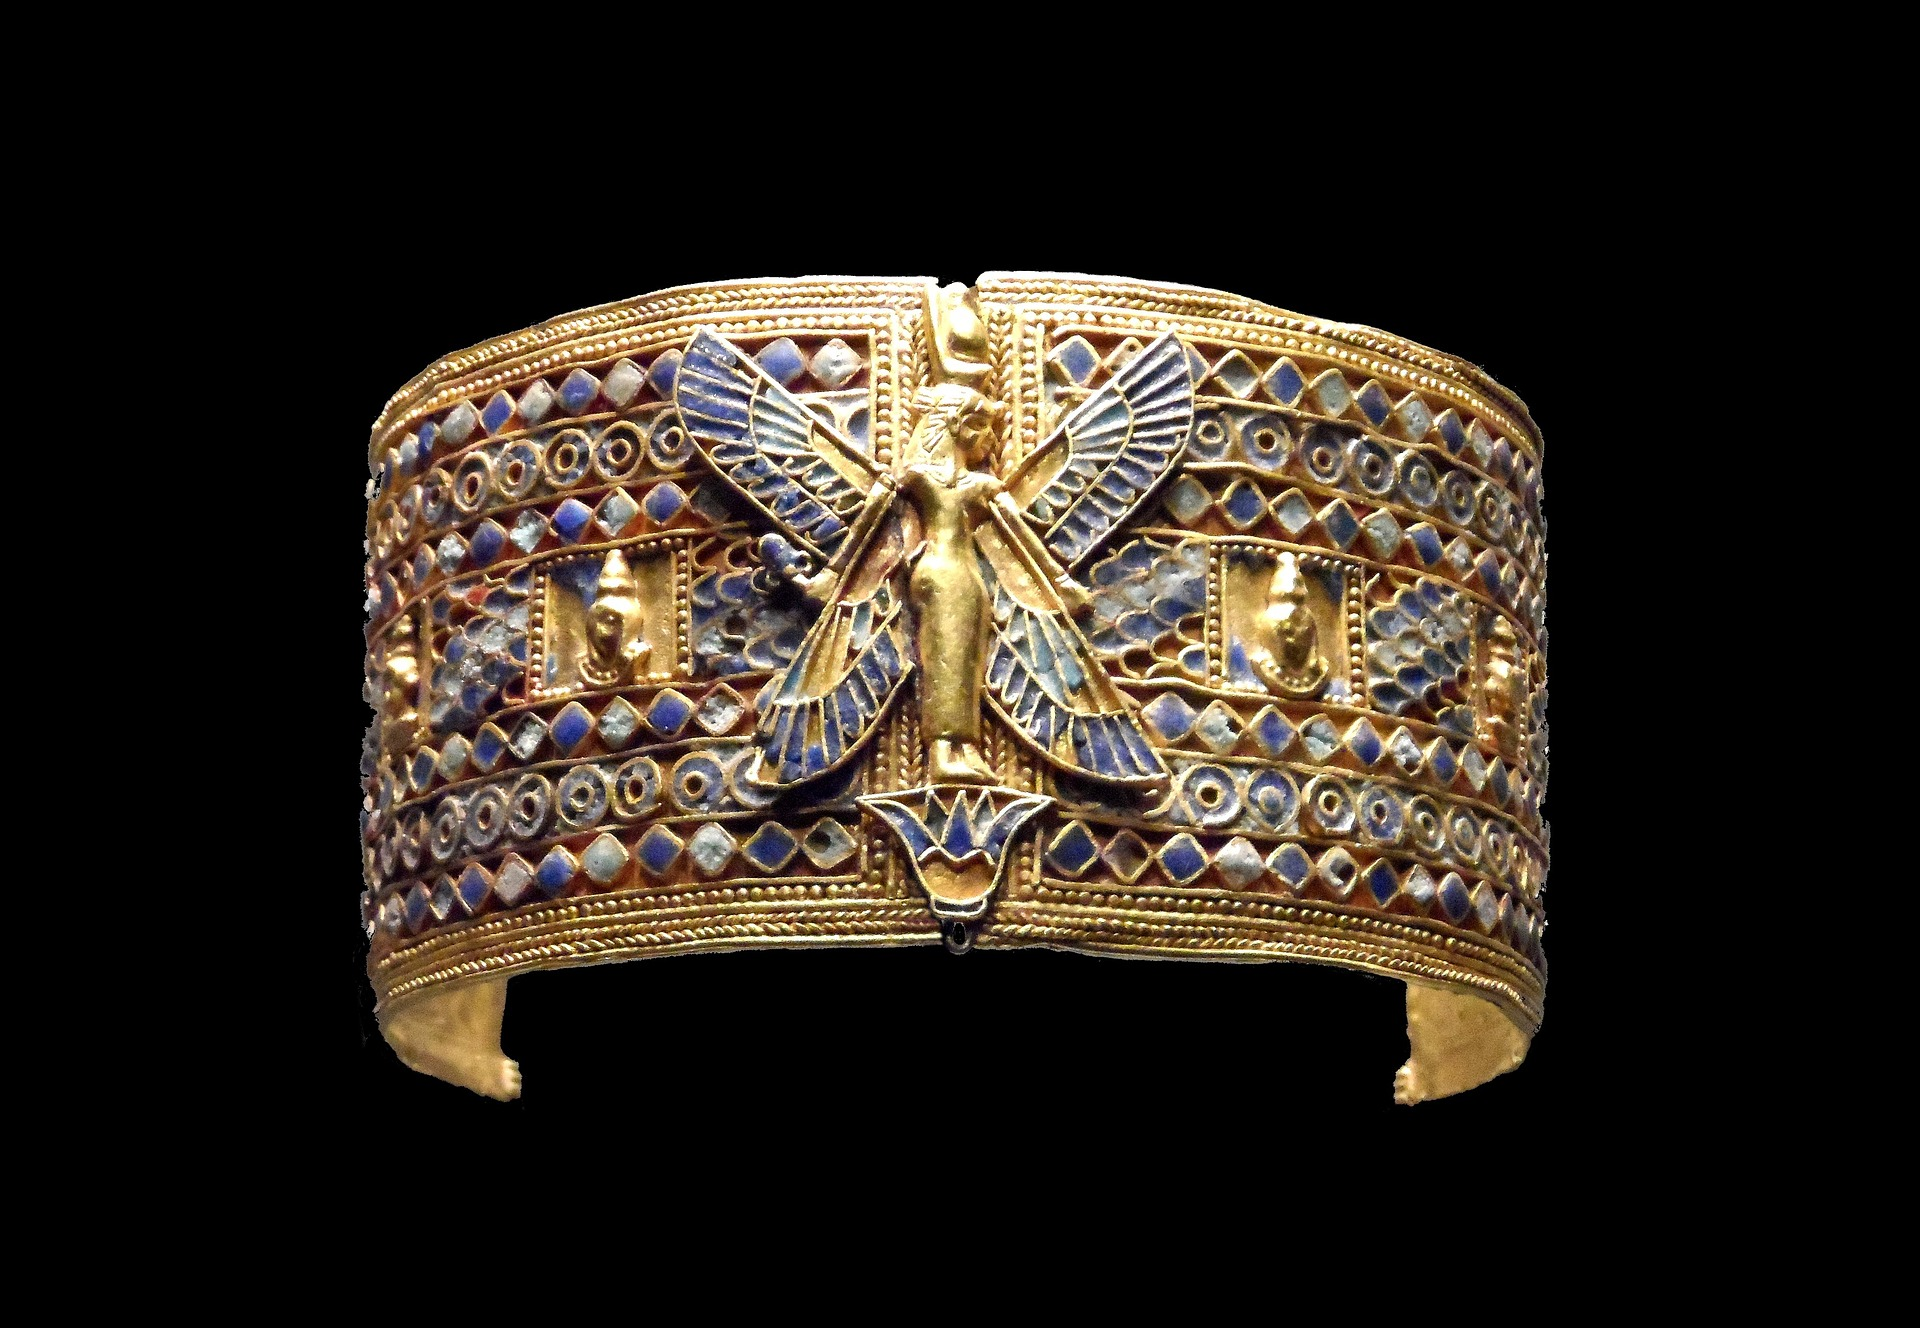
\includegraphics[width=\linewidth,keepaspectratio]{2.0.0.0_content/assets/bilder/antiker_armreif_ägypten.jpg}
    \end{column}
\end{columns}
\end{frame}

\begin{frame}{Löten bei Glas und Schmuck}
\begin{columns}[T]
    \begin{column}{0.58\textwidth}
        \small
        \begin{itemize}\setlength{\itemsep}{3mm}
            \item Eine der ältesten bekannten Anwendungen war das \textbf{Verbinden und Befestigen} von Materialien.
            \item Auch bei \textbf{Kirchenfenstern} und \textbf{Glasarbeiten} wurden einzelne Teile durch gelötete Metallverbindungen zusammengehalten.
            \item So wurde Löten schon lange vor moderner Elektronik als \textbf{praktische Verbindungstechnik} genutzt.
        \end{itemize}
        \normalsize
    \end{column}
    \begin{column}{0.42\textwidth}
        \centering
        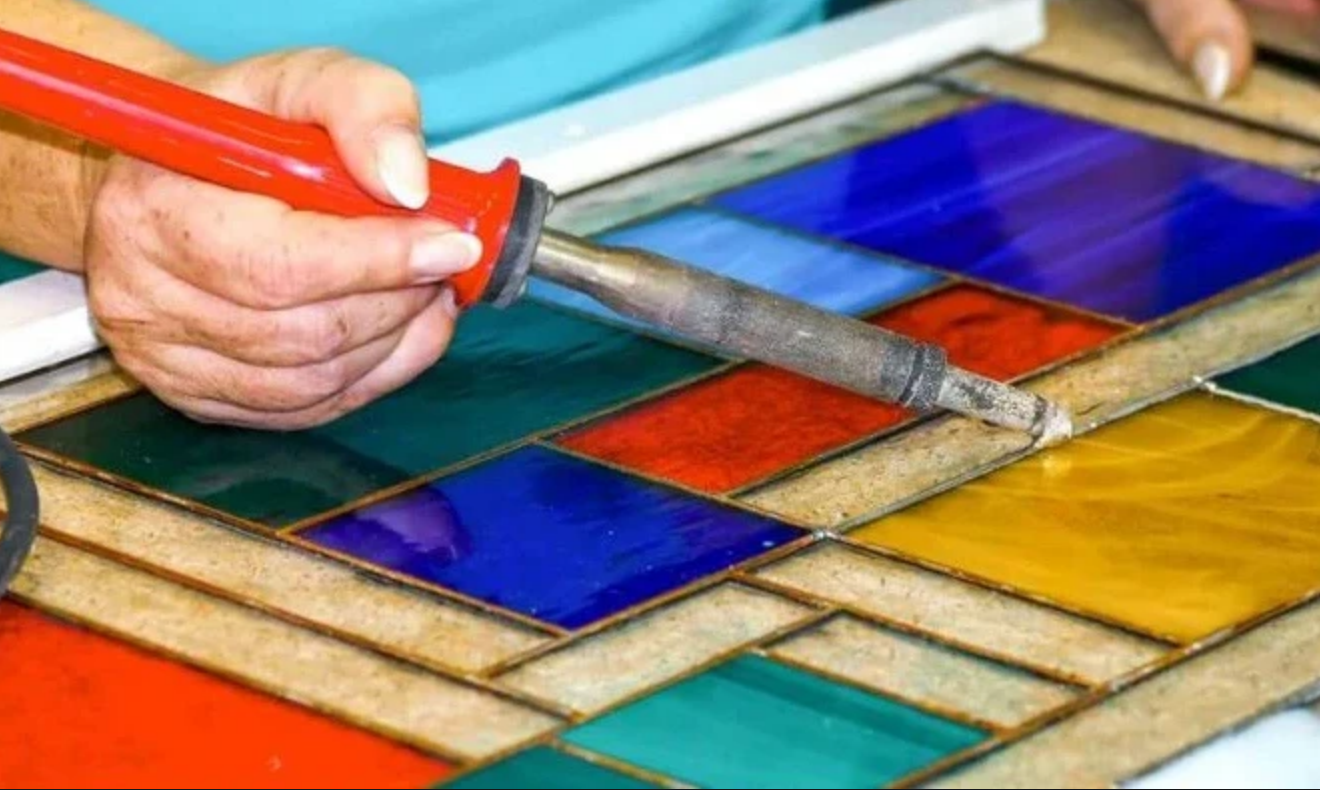
\includegraphics[width=\linewidth,keepaspectratio]{2.0.0.0_content/assets/bilder/löten_kirchenglas.png}
    \end{column}
\end{columns}
\end{frame}

\begin{frame}{Elektronik}
\begin{columns}[T]
    \begin{column}{0.58\textwidth}
        \small
        \begin{itemize}\setlength{\itemsep}{3mm}
            \item In der \textbf{Elektronikfertigung} ist Löten heute ein \textbf{Standardverfahren}.
            \item Bauteile werden so \textbf{elektrisch leitend} und zugleich \textbf{mechanisch stabil} mit einer Platine verbunden.
            \item \textbf{Handlöten} bleibt besonders wichtig bei \textbf{Prototypen}, \textbf{Reparaturen} und kleinen Projekten.
        \end{itemize}
        \normalsize
    \end{column}
    \begin{column}{0.42\textwidth}
        \centering
        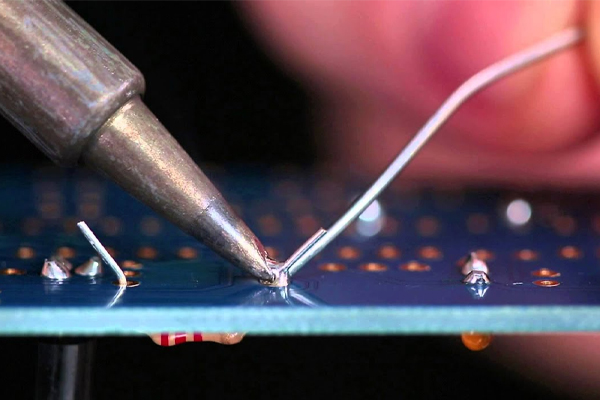
\includegraphics[width=\linewidth,keepaspectratio]{2.0.0.0_content/assets/bilder/lötstelle_mit_lötzinn.jpg}
    \end{column}
\end{columns}
\end{frame}